\section{Marco Aplicativo}

\subsection{Método de Desarrollo}

Para lograr cumplir con los objetivos planteados en el Capítulo 2, es necesario definir un
esquema o metodología de trabajo que permita la elaboración de un conjunto de
lineamientos de manera estructurada y organizada. Por lo tanto, se hace uso de el método de
Desarrollo Rápido de Aplicaciones (RAD), el cual permite la iteración rápida y continua
de pequeños objetivos para alcanzar la meta final.

RAD es un proceso de desarrollo de software que
integra un conjunto de técnicas, lineamientos y herramientas que permiten llevar a cabo, en
cortos periodos de tiempo, la implementación de funcionalidades en un sistema, de tal manera que
satisfacen las necesidades del cliente \cite{23}. Siguiendo esta metodología, el software
evoluciona y crece durante el proceso de desarrollo en base a la retro alimentación que
se tiene con el cliente. De esta manera, se realizan múltiples entregas de una tarea que
contiene las nuevas funcionalidades esperadas.

Por medio de RAD, fue posible la implementación de la solución al problema previamente planteado.
La misma está desarrollada como un servicio web API conformado por:

\begin{itemize}

\item Un modulo de extracción de revisiones de artículos wiki.

\item Un modulo de almacenamiento de datos distribuido por medio de MongoDB.

\item Un modulo de consulta de los artículos wiki extraídos y sus correspondientes revisiones.

\item Y, por último, un modulo de consulta de métricas generales de las revisiones extraídas, incluyendo: totalizaciones, promedios y moda.

\end{itemize}

La siguiente figura representa la vista general de la arquitectura de la aplicación, y como la misma interactuá con
las aplicaciones clientes que consumen el servicio:

\begin{figure}[H]
	\centering
		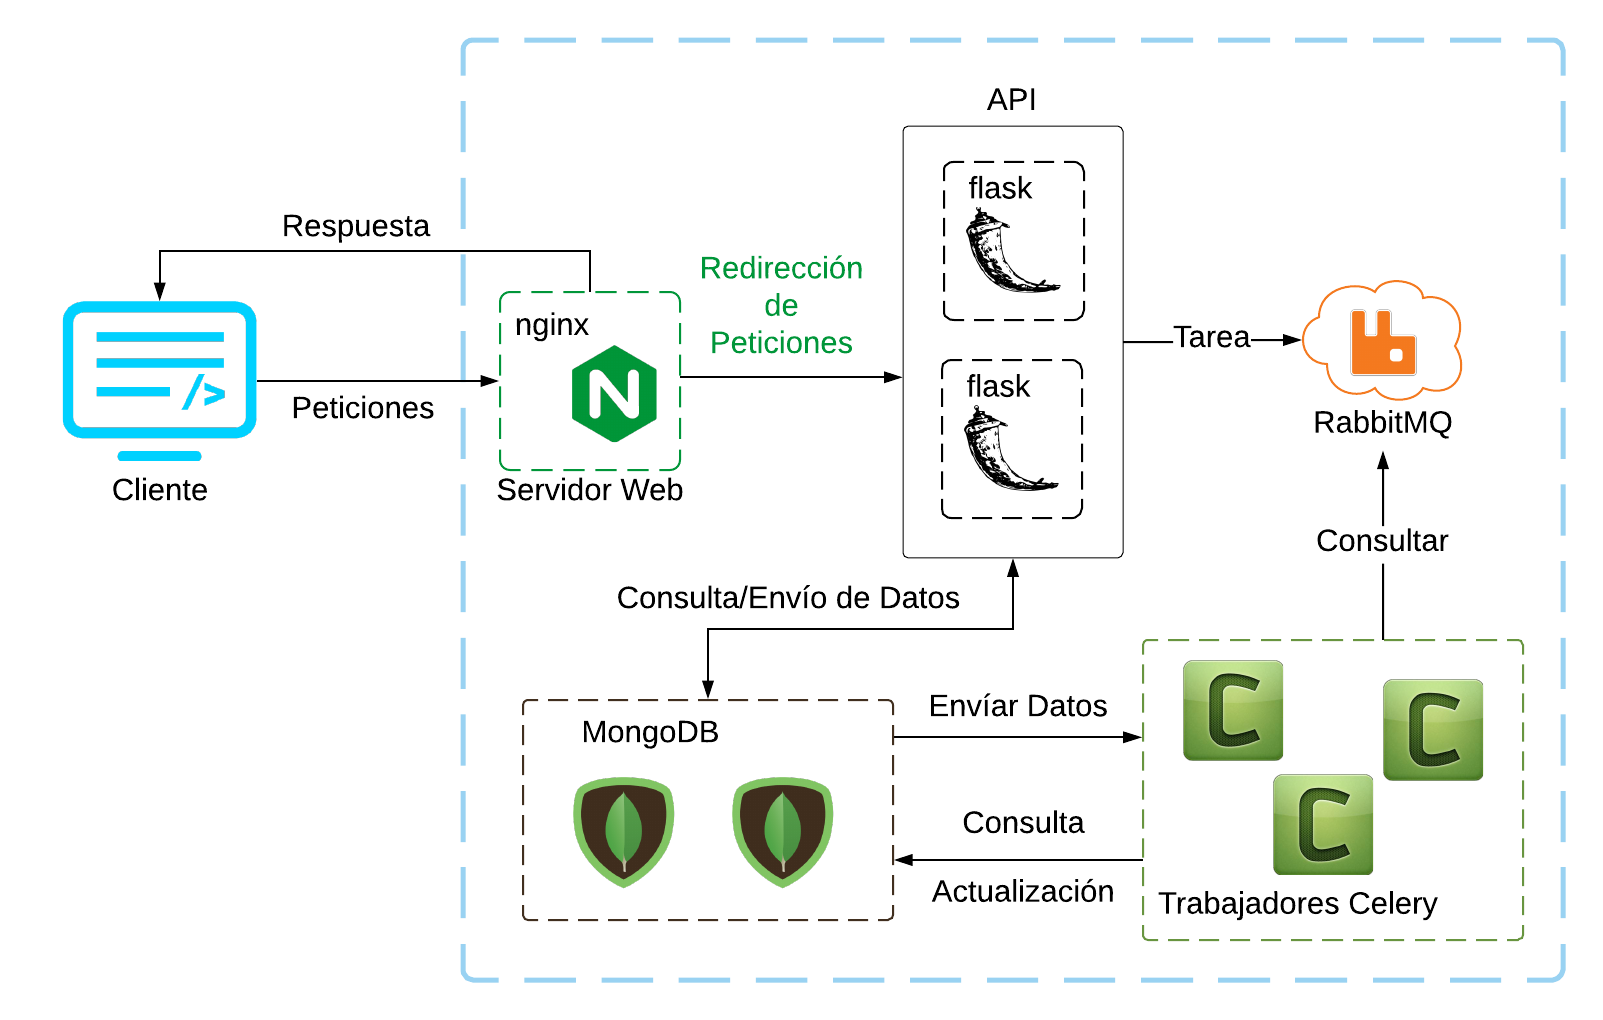
\includegraphics[width=1\textwidth]{figures/diagram_general}
	\caption{Arquitectura general de la aplicación.}
	\label{fig:diagram_general}

\end{figure}

\subsection{Servidor Web}

El servidor web que atiende las solicitudes en primera instancia es Nginx,
el cual funciona como un intermediario entre el cliente y el API que responde dicha solicitud.
Nginx permite balancear la carga de trabajo entre múltiples servidores que contienen la aplicación mediante el algoritmo de round robin,
de tal forma que cada servidor es utilizado de forma equitativa, tal como se muestra en la siguiente figura:

\begin{figure}[H]
	\centering
		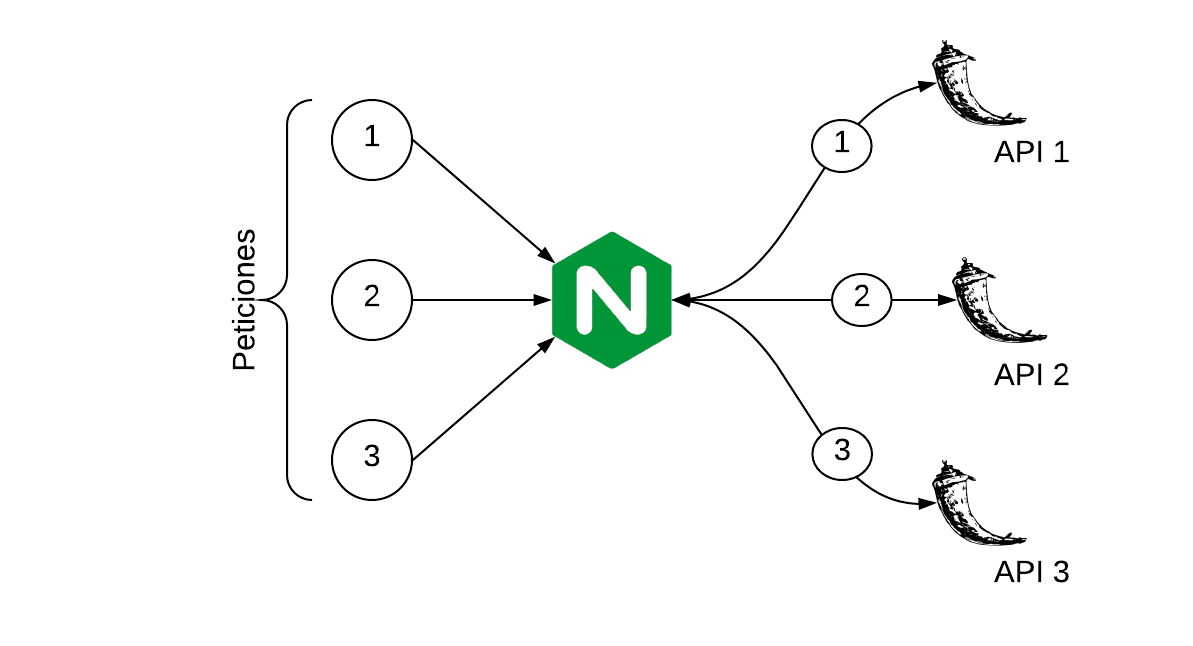
\includegraphics[width=0.9\textwidth]{figures/round_robin}
	\caption{Algoritmo de round robin para la distribución de peticiones de Nginx.}
	\label{fig:round_robin}
\end{figure}

Una vez la petición ha sido reasignada, es atendida por medio del servidor web UWSGI, y en conjunto
con Flask y el resto de las tecnologías incluidas en el API, genera una respuesta de vuelta al cliente.

\subsection{API}

El API diseñado para realizar las labores de extracción y consulta de las revisiones, hace uso del lenguaje de programación Python \texttt{2.7.10} y el uso del framework Flask \texttt{v0.12}.
Ambas tecnologías permiten la asignación de rutas específicas para cada módulo
y la atención de peticiones.

La interacción entre el servicio y una aplicación cliente puede ser apreciada en la figura \ref{fig:diagram_api_1}.

\begin{figure}[H]
	\centering
		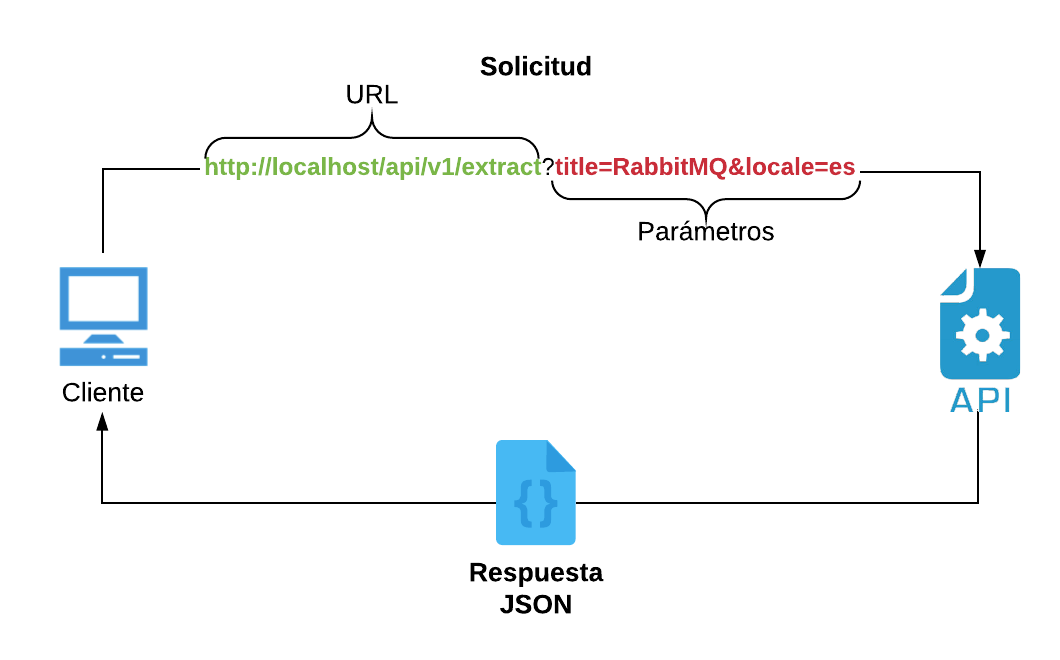
\includegraphics[width=1\textwidth]{figures/diagram_api_1}
	\caption{Interacción entre una aplicación cliente y el API.}
	\label{fig:diagram_api_1}
\end{figure}

Esta interacción se basa en la petición de un recurso o de un proceso, por parte de una aplicación cliente, a una ruta del servidor web (endpoint).
Cada petición puede incluir parámetros opcionales para la paginación, filtración de resultados, como por ejemplo, el idioma del artículo a extraer.

Las rutas de acceso que ofrece el API son las siguientes:

\begin{itemize}
	\item \texttt{/api/v1/articles}. Listado de todos los artículos extraídos.
	\item \texttt{/api/v1/revisions}. Listado de las revisiones de los artículos extraídos.
	\item \texttt{/api/v1/extract}. Extracción de revisiones de artículos wiki.
	\item \texttt{/api/v1/avg}. Cálculo del promedio de revisiones de un artículo por rango fechas.
	\item \texttt{/api/v1/count}. Cálculo de número de revisiones de un artículo por fecha.
	\item \texttt{/api/v1/mode}. Cálculo de las revisiones mas extraídas por rango de fecha.
	\item \texttt{/api/v1/status}. Indica el estado del proceso de extracción.
	\item \texttt{/api/v1/query}. Permite la ejecución de consultas personalizadas a la base de datos.
\end{itemize}

\subsubsection{Extracción de Historiales}

Para la extracción de historiales se hace uso de la ruta de acceso \texttt{/api/v1/extract}, la cual
tiene como parámetros:
\texttt{title}, que se refiere al título del del artículo; \texttt{url}, representa la ruta completa de un artículo, por ejemplo:
\texttt{https://en.wikipedia.org/wiki/The\_Lord\_of\_the\_Rings}; y por último, \texttt{locale}, el cual índica el idioma del artículo y
es completamente opcional, puesto que el sistema asume el inglés como lenguaje por defecto o lo extrae del parámetro
\texttt{url}.
Es necesario proporcionar el parámetro \texttt{url} o \texttt{title} de forma obligatoria para poder llevar a cabo la extracción.

En la siguiente figura se puede apreciar dos ejemplos del uso de los parámetros \texttt{url}, \texttt{title} y \texttt{locale}:

\begin{figure}[H]
	\centering
		
\includegraphics[width=1\textwidth]{figures/extract_url_format}
	\caption{Parámetros para la extracción de historiales.}
	\label{fig:extract_url_format}
\end{figure}

La ejecución de esta tarea se lleva a cabo por medio de Celery y RabbitMQ.
Con estas tecnologías, múltiples computadores ejecutan un proceso de Celery, los
cuales están conectados entre si gracias a RabbitMQ, escuchando constantemente los mensajes entrantes de este servicio.
Una vez recibida la petición por el API, se genera una tarea de extracción por medio de Celery, la cual tiene un identificador único. Esta tarea es encolada en una lista de
espera que es atendida por uno de los trabajadores conectados a RabbitMQ y es ejecutada en segundo plano.
Posteriormente, el API crea una respuesta a la petición generando una ruta para consultar el progreso
del proceso de extracción, la cual luce de la siguiente manera:

\begin{figure}[H]
	\centering
		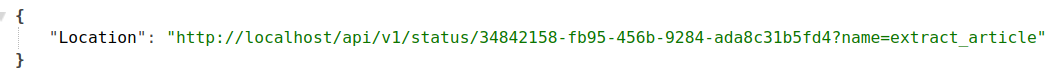
\includegraphics[width=1\textwidth]{figures/extract_response}
	\caption{Respuesta a una petición de extracción de historiales de un artículo.}
	\label{fig:extract_response}
\end{figure}

\subsubsection{Consultas}

El API consta de una ruta de acceso para consultar las revisiones extraídas y
los artículos asociados
* Revisiones
* Artículos
* Parametros de filtro
* Paginación
* Consultas AVG, COUNT, MODE
* Query

\subsection{Almacenamiento}

* MongoDB
* Sharding
* Replicas
* Nodos

\subsection{Revisita}

* Cronjob
* Minipaper, formulas

\subsection{Docker}

* Emulacion
* Nodos
* Digital Ocean?
